\chapter{Modelli teorici}

In questo capitolo investighiamo gli approcci teorici che consentono di trattare un plasma non collisionale e non neutro: ciò
vuol dire che il sistema presenta una carica netta e che le proprietà sono studiate per intervalli di tempo piccoli rispetto
alle tempistiche medie fra collisioni. Per descrivere un tale plasma possonon essere utilizzati due formalismi:
\begin{itemize}
    \item \textit{trattazione di fluido macroscopico}, basata sulle equazioni di Maxwell e sull'equazione dei momenti
    \item \textit{trattazione cinetica}, basata sulle equazioni di Vlasov-Maxwell
\end{itemize}
Nella prima delle due descrizioni vengono presi in considerazione osservabili macroscopici quali $n\left(\vec{x},\,t\right)$, 
$V\left(\vec{x},\,t\right)$ e $P\left(\vec{x},\,t\right)$: tali quantità evolvono in dipendenza dei campi elettrici e magnetici
presenti, che possono essere determinati mediante le equazioni di Maxwell. Se il plasma in analisi è freddo è possibile trascurare
le variazioni di pressione, ponendo a zero la varianza del tendore delle pressioni. Il vantaggio di un tale approccio è la sua 
elevata semplicità: in ambito fluido non è però possibile trattare instabilità collettive e fenomeni caratteristici di un plasma, 
come il Landau damping.

Per includere la fenomenologia termica nell'analisi del plasma è necessario utilizzare un approccio \textit{cinetico}: in questo
caso l'attenzione è rivolta alla distribuzione $f\left(\vec{x},\,\vec{p},\,t\right)$, che descrive la densità di probabilità di 
avere il sistema nel punto $\left(\vec{x},\,\vec{p}\right)$ dello spazio delle fasi al tempo $t$. Per come è definita la
distribuzione $f$, abbiamo che
$$f\left(\vec{x},\,\vec{p},\,t\right)d^3xd^3p\,=\,\text{numero medio di particelle nell'intorno di } \left(\vec{x},\,\vec{p}\right)$$
Questo approccio consente di studiare un'ampia classe di fenomeni collettivi che dipendono dalla struttura della distribuzione
all'equilibrio nello spazio delle fasi.

\section{Trattazione cinetica}

Consideriamo un plasma non neutro di elettroni caratterizzati da carica $e$ e massa $m$: per scale di tempo corte rispetto
al tempo di collisione la funzione di distribuzione di singola particella $f\left(\vec{x},\,\vec{p},\,t\right)$ evolve secondo
l'equazione di Vlasov, che descrive l'evoluzione incomprimibile secondo il teorema di Liouville nello spazio delle fasi
6-dimensionale $\left(\vec{x},\,\vec{p}\right)$.
\begin{equation}
    \left\{\frac{\partial}{\partial t}\,+\,\vec{v}\cdot\frac{\partial}{\partial \vec{x}}\,+\,e\left(\vec{E}\,+\,\frac{\vec{v}\times\vec{B}}{c}\right)\cdot\frac{\partial}{\partial \vec{p}}\right\}f\left(\vec{x},\,\vec{p},\,t\right)\,=\,0
    \label{equation: VlasovEq}
\end{equation}
Notiamo che è presente un termine in cui figurano sia il campo elettrico che il campo magnetico: possiamo determinarli utilizzando le
equazioni di Maxwell
\begin{align}
    &\nabla \times \vec{E} = -\frac{1}{c}\left[c\right]\frac{\partial \vec{B}}{\partial t} \\
    &\nabla \times \vec{B} = \frac{4\pi}{c}\left[\frac{\mu_0 c}{4\pi}\right]e\int{d^3p\vec{v}f(\vec{x},\,\vec{p},\,t)} + \frac{4\pi}{c}\left[\frac{\mu_0 c}{4\pi}\right]\vec{J}_{ext} + \frac{1}{c}\left[\frac{1}{c}\right] + \frac{\partial \vec{E}}{\partial t} \\
    &\nabla \cdot \vec{E} = 4\pi\left[\frac{1}{4\pi\varepsilon_0}\right]e\int{d^3p f\left(\vec{x},\,\vec{p},\,t\right)} + 4\pi\left[\frac{1}{4\pi\varepsilon_0}\right]\rho_{ext} \\
    &\nabla \cdot \vec{B} = 0
\end{align}
Le equazioni di Vlasov-Maxwell sono altamente non lineari, in quanto $f\left(\vec{x},\,\vec{p},\,t\right)$ è modificata dai campi auto-indotti
dal plasma, che a loro volta evolvono quando la funzione di distribuzione cambia. In condizioni di stato quasi-stazionario è possibile
porre a zero tutte le derivate parziali rispetto al tempo in modo da determinare le soluzioni stazionarie $f^0\left(\vec{x},\,\vec{p}\right)$,
$\vec{E}^0\left(\vec{x}\right)$ e $\vec{B}^0\left(\vec{x}\right)$: lavorando con piccole perturbazioni è possibile valutare la stabilità
degli equilibri così individuati.

\section{Trattazione fluida}

In alcune circostanze il comportamento globale del plasma può essere descritto utilizzando un'approccio fluido-dinamico: 
siamo interessati alla densità del sistema $n\left(\vec{x},\,t\right)$, alla velocità media $\vec{V}\left(\vec{x},\,t\right)$,
al momento medio $\vec{P}\left(\vec{x},\,t\right)$ ed al tensore delle pressioni $\mathbf{P}\left(\vec{x},\,t\right)$. Per 
passare dalla trattazione cinetica a quella fluida introduciamo i primi momenti della distribuzione $f\left(\vec{x},\,\vec{p},\,t\right)$ 
integrando nei momenti, in modo tale da perdere l'informazione cinetica e mantenere solo quella spaziale. Possiamo quindi 
riconoscere:
\begin{equation}
    n\left(\vec{x},\,t\right)\,=\,\int d^3p \,f\left(\vec{x},\,\vec{p},\,t\right)
    \label{equation: numb_density}
\end{equation}
\begin{equation}
    n\left(\vec{x},\,t\right)\vec{V}\left(\vec{x},\,t\right)\,=\,\int d^3p\,\vec{v} f\left(\vec{x},\,\vec{p},\,t\right)
    \label{equation: mean_velocity}
\end{equation}
\begin{equation}
    n\left(\vec{x},\,t\right)\vec{P}\left(\vec{x},\,t\right)\,=\,\int d^3p\,\vec{p} f\left(\vec{x},\,\vec{p},\,t\right)
    \label{equation: p_tens}
\end{equation}
\begin{equation}
    \mathbf{P}\left(\vec{x},\,t\right)\,=\,\int d^3p\left[\vec{p}\,-\,\vec{P}\left(\vec{x},\,t\right)\right]\left[\vec{v}\,-\,\vec{V}\left(\vec{x},\,t\right)\right] f\left(\vec{x},\,\vec{p},\,t\right)
    \label{equation: p_tens1}
\end{equation}
Possiamo ora ottenere le equazioni fluide andando ad integrare nei momenti: la semplice integrazione in $d^3p$ restituisce 
l'equazione di continuità, mentre lavorando con $\vec{p}d^3p$ è possibile ottenere l'equazione che descrive l'equilibrio delle
forze:
\begin{equation}
    \frac{\partial n}{\partial t}\,+\,\nabla \cdot \left(n\vec{V}\right)\,=\,0
    \label{equation: continuity_eq}
\end{equation}
\begin{equation}
    n\left(\frac{\partial}{\partial t}\,+\,\vec{V}\cdot \nabla\right)\vec{P}\,+\,\nabla \cdot \mathbf{P}\,=\,nq\left(\vec{E}\,+\,\frac{1}{c}\left[c\right]\vec{v} \times \vec{b}\right)
    \label{equation: force_balance}
\end{equation}
Abbiamo trovato un sistema di equazioni differenziali in cui nell'equazione che descrive l'evoluzione del momento di ordine 0 
compare il momento di primo ordine ed in generale nell'equazione riguardante il k-esimo momento è presente il k+1-esimo: per 
chiudere il sistema supponiamo di trattare un plasma freddo, ossia caratterizzato da velocità termica molto inferiore alla 
velocità fluida in gioco. Così facendo possiamo trascurare il termine di ordine superiore, ossia la divergenza del tensore delle 
pressioni, di fatto trascurando l'agitazione termica rispetto ai moti del fluido.

\section{Equilibrio di rotazione}

Consideriamo un plasma non-neutro di lunghezza infinita confinato radialmente da un campo magnetico $\vec{B}\,=\,B_0 \hat{e}_z$: 
in condizioni di stato stazionario $\left(\partial/\partial t\,=\,0\right)$ supponiamo di avere un profilo di densità a gradino 
assi-simmetrico del tipo:
\begin{equation}
    n\left(r\right)\,=\,
\begin{cases}
    n_0 \qquad \qquad r \in \left[0,\,r_b\right] \\
    0\,\,\, \qquad \qquad r \in \left(r_b,\,\infty\right)
\end{cases}
\label{equation: eq_density}
\end{equation}
\begin{figure}[H]
    \centering
    \includegraphics[width=0.9\textwidth]{Immagini/ProfiliDensità.png}
    \caption{Confronto fra profilo di densità ideale e situazione realistica}
    \label{figure: ProfDens}
\end{figure}
La distribuzione spaziale di carica genera un campo elettrico diretto radialmente ed identicamente nullo nel centro del 
plasma: è possibile determinare l'andamento di tale campo risolvendo l'equazione di Poisson. Il set di equazioni che consente 
di descrivere la situazione in analisi è:
\begin{equation}
    \nabla \cdot \left(n\vec{V}\right)\,=\,0
    \label{equation: conteq_steadystate}
\end{equation}
\begin{equation}
    \left(\vec{V}\cdot \nabla\right)\vec{V}\,=\,\frac{q}{m}\left(-\nabla\Phi\,+\,\frac{1}{c}\left[c\right]\vec{v} \times \vec{b}\right)
    \label{equation: forcebalance_steadystate}
\end{equation}
\begin{equation}
    \nabla^2\Phi\,=\,-4\pi\left[\frac{1}{4\pi\varepsilon_0}\right]qn
    \label{equation: Poisson_steadystate}
\end{equation}
Procediamo con l'obiettivo di determinare il potenziale: sfruttiamo le simmetrie del sistema, evidenti nel set di coordinate
cilindriche $\left(r,\,\theta,\,z\right)$. Dato che non abbiamo dipendenza dalla coordinata $z$, tutte le derivate rispetto alla 
quota saranno identicamente nulle. L'equazione di continuità e l'equazione di evoluzione dei momenti si traducono in:
\begin{align}   % FARE UN CHECK: INDICI POTREBBERO ESSERE ERRATI
    & \frac{1}{r}\frac{\partial}{\partial r}\left(rnV_z\right)\,+\,\frac{1}{r}\frac{\partial}{\partial \theta}\left(nV_\theta\right)\,=\,0 \\
    & V_r\frac{\partial V_z}{\partial r}\,+\,\frac{V_\theta}{r}\frac{\partial V_z}{\partial V_\theta}\,-\,\frac{V^2_\theta}{r}\,=\,\frac{q}{m}\left(-\frac{\partial \Phi}{\partial r}\,+\,\frac{1}{c}\left[c\right]V_\theta B_\theta\right) \\
    & V_r\frac{\partial V_\theta}{\partial r}\,+\,\frac{V_\theta}{r}\frac{\partial V_\theta}{\partial \theta}\,+\,\frac{V_\theta V_r}{r}\,=\,-\frac{q}{m}\left(\frac{1}{r}\frac{\partial \Phi}{\partial \theta}\,+\,\frac{1}{c}\left[c\right]V_zB_\theta\right) \\
    & \frac{1}{r}\frac{\partial}{\partial r}\left(r\frac{\partial \Phi}{\partial r}\right)\,+\,\frac{1}{r^2}\frac{\partial^2\Phi}{\partial \theta ^2}\,=\,-4\pi\left[\frac{1}{4\pi\varepsilon_0}\right]qn
\end{align}
Specializzando la casistica in analisi sfruttando il profilo di densità introdotto in precedenza \eqref{equation: eq_density} ed imponendo 
delle ulteriori condizioni di simmetria sulla velocità:
\begin{equation}
\begin{cases}
    n\,=\,n\left(r\right) \\
    V_r\,=\,0   \\
    V_\theta\,=\,V_\theta\left(r\right)
\end{cases}
\end{equation}
è possibile ridurre il set di partenza a sole due equazioni che consentono di ottenere infomazioni riguardo al comportamento 
globale del plasma. 
\begin{figure}[H]
    \centering
    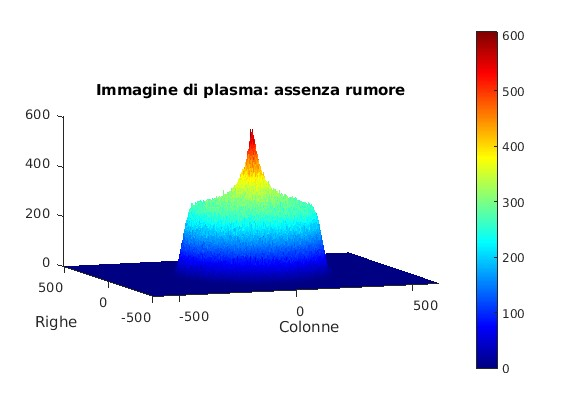
\includegraphics[width=0.9\textwidth]{Immagini/RealPlasma.jpg}
    \caption{Immagine di plasma scattata in laboratorio dove notiamo come il profilo di densità risulti alquanto lontano dalle
    condizioni di idealità. }
    \label{figure: RealPlasma}
\end{figure}
Noto il profilo di densità, risolviamo inizialemente il problema di Poisson per poi ottenere delle informationi 
sulla velocità azimutale, che sarà quella caratteristica di un moto di rotazione rigida. Procediamo con l'analisi delle equazioni 
ridotte per merito delle assunzioni precedentemente giustificate:
\begin{equation}
    -\frac{V_\theta^2}{r}\,=\,\frac{q}{m}\left(-\frac{\partial \Phi}{\partial r}\,+\,\frac{1}{c}\left[c\right]V_\theta B_\theta\right)
    \label{equation: reduced_Poisson}
\end{equation}
\begin{equation}
    \frac{1}{r}\frac{\partial}{\partial r}\left(r\frac{\partial \Phi}{\partial r}\right)\,=\,-4\pi\left[\frac{1}{4\pi\varepsilon_0}\right]qn
    \label{equation: reduced_momentum}
\end{equation}
L'equazione \eqref{equation: reduced_momentum} deve essere risolta separatamente nelle due regioni in cui può essere diviso lo spazio 
utilizzando come criterio la densità di carica:
\begin{equation}
    \frac{1}{r}\frac{\partial}{\partial r}\left(r\frac{\partial \Phi}{\partial r}\right)\,=\,
    \begin{cases}
        \alpha n_0 \,\,\,\, \qquad \qquad r \in \left[0,\,r_p\right] \\
        0 \qquad \qquad \qquad r \in \left[r_p,\,r_W\right]
    \end{cases}
    \label{equation: Poisson_step1}
\end{equation}
dove la costante alfa è definita come
\begin{equation}
    \alpha\,=\,4\pi e\left[\frac{1}{4\pi\varepsilon_0}\right]
\end{equation}
Per avere un problema ben definito è necessario imporre delle condizioni al contorno di senso fisico: vogliamo evitare una 
soluzioni divergente richiedendo che
\begin{equation}
    \begin{cases}
    \Phi \left(r\,=\,r_W\right)\,=\,0, \\
    \Phi \left(r\,=\,0\right)\,<\,\infty.
    \end{cases}
    \label{equation: BC}
\end{equation}
Integrando il problema di Poisson in entrambe le regioni prese in considerazione ed imponendo continuità e derivabilità in 
$r\,=\,r_p$ per giuntare le soluzioni si ottiene che
\begin{equation}
    \Phi\left(r\right)\,=\,\frac{m}{e}\omega_p^2
    \begin{cases}
        \frac{r^2\,-\,r_p^2}{4}\,+\,\frac{r_p^2}{2}\log{\left(\frac{r_p}{r_w}\right)}   \\
        \frac{r_p^2}{2}\log{\left(\frac{r}{r_W}\right)}
    \end{cases}
    \label{equation: potential_solution}
\end{equation}
dove si indica con $\omega_p^2$ la frequenza di plasma elettronico, data da
\begin{equation}
    \omega_p^2\,=\,\frac{\alpha e n_0}{m}.
    \label{equation: plasma_freq}
\end{equation}
Ricavare il campo dall'equazione \eqref{equation: potential_solution} è banale: noto $\vec{E}$, è possibile andarlo a sostituire nell'equazione 
per l'evoluzione dei momenti ottendo che
\begin{equation}
    -m\omega^2r\,=\,\frac{m}{2}\omega_p^2r\,-\,\left(\frac{eB_0}{mc}\left[c\right]\right),
    \label{equation: momentum_eq1}
\end{equation}
dove $\omega$ è una frequenza angolare introdotta per esplicitare $V_\theta\left(r\right)\,=\,\omega\left(r\right)r$. Possiamo
riconoscere la frequenza angolare di ciclotrone, che evidenzia quale sia la frequenza di rotazione attorno alle linee di campo
magnetico:
\begin{equation}
    \Omega\,=\,\frac{eB_0}{mc}\left[c\right].
    \label{equation: ciclotron_frequency}
\end{equation}
La condizione esplicitata dall'equazione \eqref{equation: momentum_eq1} è verificata solamente quando si verifica che
\begin{equation}
    \omega^2\,-\,\Omega\omega\,+\,\frac{\omega_p^2}{2}\,=\,0,
    \label{equation: omega_condition}
\end{equation}
le cui soluzioni sono
\begin{equation}
    \omega^\pm\,=\,\frac{\Omega}{2}\left(1\,\pm\,\sqrt{1\,-\,s}\right), 
    \label{equation: omega_solution}
\end{equation}
dove $s\,=\,2\omega_p^2/\Omega^2$ è il parametro di auto-campo: tale quantità esplicita il rapporto fra la forza elettrostatica
 che tende a defocalizzare il plasma e la forza di natura magnetica che ha un effetto focalizzante. Notiamo che l'equazione di 
secondo grado \eqref{equation: omega_condition} ammette soluzione solo se $s \leq 1$: per avere un plasma in rotazione rigida è
necessario che siano più intense le forze di natura magnetica legate all'applicazione di un campo esterno. La condizione per cui 
$s\,=\,1$ è nota come \textit{limite di Brillouin}: per avere un plasma confinato è necessario che
\begin{equation}
    \frac{n_0 mc^2}{\frac{B_0}{8\pi}\left[\frac{4\pi}{\mu_0}\right]}\,\leq\,1
    \label{equation: confinement_cond}
\end{equation}
e di conseguenza è presente una densità limite oltre la quale la repulsione elettrostatica vince ed il plasma si disgrega. 
\begin{figure}[H]
    \centering
    \includegraphics[width=0.9\textwidth]{Immagini/VelocitàAngolari.png}
    \caption{Relazione per la determinazione di $\omega$: il ramo superiore corrisponde alla soluzione $\omega^+$, mentre
    quello inferiore ad $\omega^-$}
    \label{figure: ProfDens}
\end{figure}
Noi lavoreremo con $s \ll 1$ a causa della bassa densità dei plasmi prodotti in laboratorio: saremo in particolare interessati 
a regimi di rotazione lenta.

\section{Traiettorie delle singole particelle}

\'E interessante esaminare i movimenti delle singole particelle costituenti il plasma: un elettrone percepisce l'azione di 
forze di natura elettro-magnetica prodotte dal campo elettrico auto-indotto e dal campo magnetico esterno, che stiamo continuando 
a considerare diretto lungo l'asse z.
